\section{Results}
\label{sec:results}

% EXAMPLE content -- numbers are \val... macros from paper/generated/values.tex.

At $\sqrts = \valSqrtSRef$ the total cross section from \cref{eq:sigmatot} is
$\sigma = \valSigmaTotMma$. Integrating \cref{eq:dsigma} numerically in Python
gives $\valSigmaTotNum$, a relative difference of $\valSigmaRelDiff$, and a
forward--backward asymmetry $A_\text{FB} = \valAFB$ as expected for pure QED.
The angular distribution is shown in \cref{fig:dsigma}.

\begin{figure}[t]
  \centering
  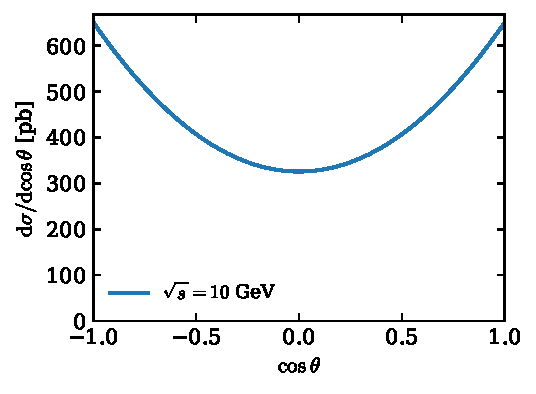
\includegraphics{ee_mumu_dsigma}
  \caption{Angular distribution of $e^+e^-\to\mu^+\mu^-$ at $\sqrts=\valSqrtSRef$.}
  \label{fig:dsigma}
\end{figure}
